% Stand-alone preview of Habib Hasanov's report sections (NOT the submitted report).
% Build from docs/report/:  latexmk -pdf -outdir=build hasanov_preview.tex
% The final IEEEtran report includes the same section files (see README_HabibHasanov.md).
\documentclass[10pt,twocolumn]{article}
\usepackage[margin=0.75in]{geometry}
\usepackage{graphicx,amsmath,amssymb,url,booktabs}
\usepackage[hidelinks]{hyperref}
\graphicspath{{../diagrams/}{../../results/figures/}}
\title{INFT 6000 HW3 --- Group 4\\\large Preview: Sections 4, 5 and 7.4 (Habib Hasanov)}
\author{Habib Hasanov}\date{}
\begin{document}
\maketitle
% Stand-in labels for sections written by other members (defined in their files).
\makeatletter
\def\hhstub#1#2{\expandafter\gdef\csname r@#1\endcsname{{#2}{}{}{}{}}}
\hhstub{sec:architecture}{2}\hhstub{sec:consistency}{3}\hhstub{sec:cap}{6}\hhstub{sec:setup}{7.1}
\makeatother
\setcounter{section}{3}
% Section 4 - Conflict Resolution and Anti-Entropy (Habib Hasanov)
% Figure: ../diagrams/antientropy_merkle.png (docs/diagrams/hasanov_diagrams.py)
% Citations: docs/references.bib
\section{Conflict Resolution and Anti-Entropy}\label{sec:antientropy}

Section~\ref{sec:consistency} showed that a write reaches all live replicas but is
acknowledged by only $W$ of them, so replicas can disagree after any failure. This section
explains how Cassandra decides \emph{which} version is correct (conflict resolution) and how
replicas that missed writes are brought back in line (anti-entropy). Experiment~4
(Section~\ref{sec:results-exp46}) isolates each mechanism.

\subsection{Last-write-wins per cell}

Every cell (one column of one row) carries a 64-bit write timestamp in microseconds. Our
driver assigns it on the client; \texttt{USING TIMESTAMP} overrides it, and without a client
value the coordinator assigns one. Whenever two versions of a cell meet---in a read, a hint,
read repair, repair streaming or compaction---the higher timestamp wins and the other version
is discarded~\cite{lakshman2010cassandra,cassdoc-dynamo}. Ties are broken deterministically: a
deletion beats a live value, and between two live values the byte-wise larger value wins,
so every replica independently reaches the same result without communicating. Because
reconciliation is per \emph{cell}, concurrent updates to different columns of one row both
survive; only updates to the same cell conflict.

Last-write-wins (LWW) makes physical clocks part of correctness. Timestamps are not
Lamport clocks~\cite{lamport1978time}: they do not capture causality, so a writer whose clock
runs ahead can win against a later write, and two causally ordered writes from different
clients can be reordered by skew. Production clusters therefore rely on NTP-synchronised
clients and nodes. In our testbed all containers share the host clock, which removes skew
from the measurements; Experiment~5 instead \emph{sets} timestamps with \texttt{USING
TIMESTAMP} to make the winner deterministic.

\paragraph{Why not vector clocks?}
Dynamo tracks causality with vector clocks~\cite{decandia2007dynamo,mattern1989vector}: when
two versions are concurrent, both are kept as \emph{siblings} and the application merges them
on its next read. Cassandra deliberately dropped this~\cite{lakshman2010cassandra}. LWW needs no
per-key version metadata that grows with the number of writers, no read-time merge logic in
every client, and no sibling explosion under contention, and it composes with the
log-structured storage engine: compaction can merge SSTables with a simple timestamp
comparison. The price is that \emph{concurrent} writes to the same cell are not detected:
one acknowledged write silently disappears. Experiment~5 shows this for a partition, and
the plain-\texttt{INSERT} race of Experiment~6 for concurrent clients; applications that cannot
tolerate it use lightweight transactions (Section~\ref{sec:consensus}) or counters.

\paragraph{Deletes are writes}
A \texttt{DELETE} writes a \emph{tombstone}, a timestamped marker that wins over older
values like any other cell. Tombstones are purged by compaction only after the table's
\texttt{gc\_grace\_seconds} (default 864\,000\,s, ten days)~\cite{cassdoc-tombstones}. If a
replica misses a delete and is not repaired before the tombstone is purged elsewhere, the
replica's old value is later streamed back as a ``zombie''---the deleted row reappears. Every
replica must therefore be repaired at least once per \texttt{gc\_grace\_seconds}, which is
the hard operational requirement behind the mechanisms below.

\subsection{Three repair mechanisms}

Fig.~\ref{fig:antientropy} and Table~\ref{tab:antientropy} compare the mechanisms. They differ in
what triggers them, what data they cover, and whether they can be relied on.

\begin{figure*}[t]\centering
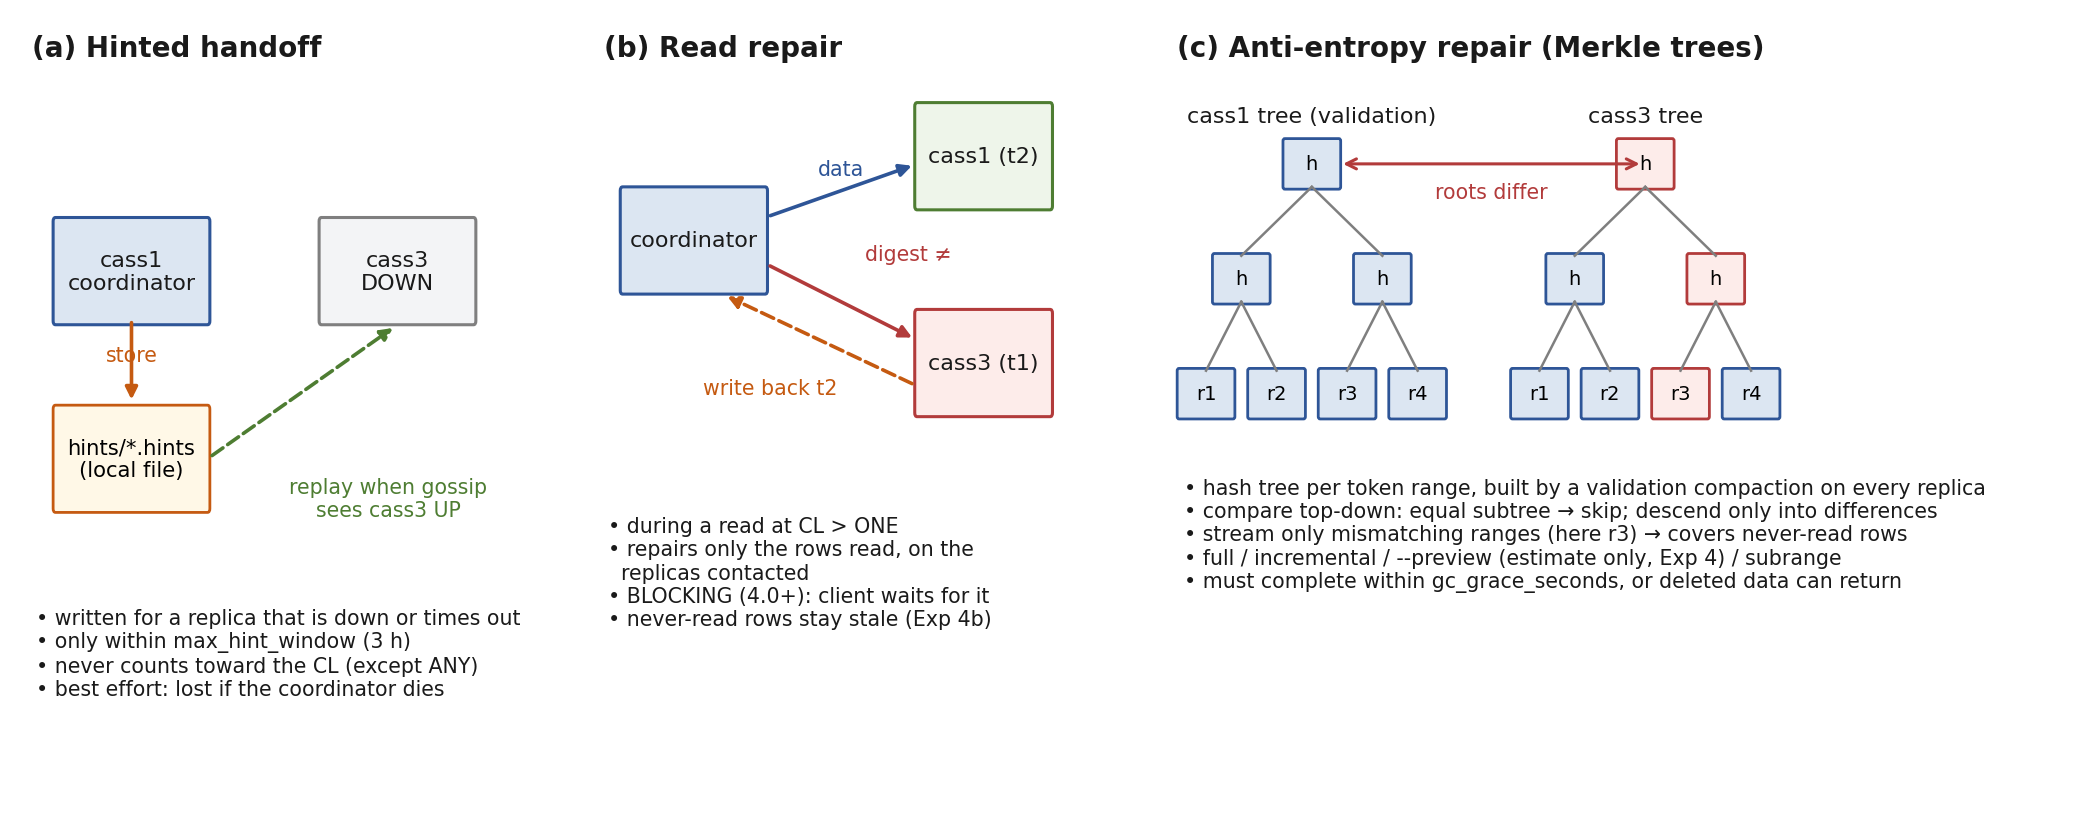
\includegraphics[width=0.92\textwidth]{antientropy_merkle.png}
\caption{Cassandra's three repair mechanisms: (a) hints written by the coordinator for a down
replica, (b) read repair on a digest mismatch, (c) Merkle-tree anti-entropy repair, which
narrows a mismatch to the token sub-ranges that must be streamed.}\label{fig:antientropy}
\end{figure*}

\paragraph{Hinted handoff}
When a coordinator sends a mutation to a replica that gossip reports as down, or that does
not acknowledge in time, it stores a \emph{hint} (target host ID plus mutation) in its local
\texttt{hints} directory; hints are buffered in memory and flushed to files periodically
(\texttt{hints\_flush\_period}, 10\,s). When gossip marks the target up again, the
coordinator streams the hints to it, throttled, and deletes each file once delivered.
Hints are written only while the target has been down for less than
\texttt{max\_hint\_window} (3\,h by default) and expire with the table's
\texttt{gc\_grace\_seconds}~\cite{cassdoc-hints}. They are a best-effort optimisation:
they never count towards the consistency level (except ANY,
Section~\ref{sec:consistency}), they are lost if the coordinator itself fails before
delivery, and a replica down longer than the window receives none.

\paragraph{Read repair}
During a read at a level that contacts more than one replica, the coordinator compares a
data response with digests; on a mismatch it fetches full data, reconciles by LWW and
writes the winning cells back to the stale replicas it contacted. Since 4.0 this is
\emph{blocking}: the client is answered only after the repair writes are acknowledged, which
makes successive quorum reads monotonic (Section~\ref{sec:consistency}). The
probabilistic background variant (\texttt{read\_repair\_chance}) was removed in 4.0 and
replaced by the per-table \texttt{read\_repair} option (\texttt{BLOCKING} or
\texttt{NONE})~\cite{cassdoc-readrepair}. Read repair is \emph{opportunistic}: it repairs only
rows that are read, at a level above ONE, on the replicas that the read touched. Rows that are
never read stay divergent, which Experiment~4b demonstrates with a control sample.

\paragraph{Anti-entropy repair}
\texttt{nodetool repair} compares whole token ranges. Each replica of a range runs a
\emph{validation compaction} that hashes its data into a Merkle tree~\cite{merkle1987}:
leaves cover contiguous token sub-ranges and every inner node hashes its children. The
initiator compares the trees top-down; equal subtrees are skipped, so only sub-ranges whose
leaf hashes differ are streamed between replicas, and LWW reconciles the streamed data on
arrival. This is the only mechanism that covers \emph{all} data, including never-read rows
and missed deletes. \emph{Full} repair rebuilds trees over all SSTables; \emph{incremental}
repair (the default command since 2.2, made reliable in 4.0) validates only SSTables not yet
marked repaired and then anti-compacts them into a repaired set; \texttt{-pr} limits a node
to its primary ranges and \texttt{-st}/\texttt{-et} to a subrange~\cite{cassdoc-repair}.
\texttt{--preview} builds and compares the trees but only reports the streaming that would
occur~\cite{cass13257}; Experiment~4 uses it as a non-invasive divergence detector before
and after each mechanism. Repair costs disk and network I/O proportional to the data, so in
5.0 it is scheduled by the operator (or an external tool). Cassandra 6.0 adds a built-in
scheduler (CEP-37~\cite{cep37,cassdoc-autorepair}); it is disabled by default and was not
available in our 5.0.8 cluster.

\begin{table}[t]\centering\footnotesize
\caption{Repair mechanisms in Cassandra 5.0.}\label{tab:antientropy}
\begin{tabular}{@{}p{0.2\columnwidth}p{0.22\columnwidth}p{0.22\columnwidth}p{0.24\columnwidth}@{}}\hline
 & Hinted handoff & Read repair & Anti-entropy repair \\ \hline
Trigger & write to a down / slow replica & digest mismatch in a read at CL $>$ ONE & operator / scheduler \\
Scope & writes missed during $\le$ 3\,h & rows read, replicas contacted & all data of the repaired ranges \\
Timing & on recovery (gossip UP) & inline, blocks the read & offline batch \\
Guarantee & best effort & read rows monotonic & complete if it finishes \\
Cost & hint storage on coordinator & extra read latency & validation compaction + streaming \\ \hline
\end{tabular}
\end{table}

\paragraph{How they combine}
The mechanisms are layered by cost. Hints repair short outages almost for free; read repair
fixes hot data on the critical path; anti-entropy is the safety net that bounds divergence in
time and makes deletes durable. None of them changes what a client can observe at
$R + W > N$---that guarantee comes from quorum intersection
(Section~\ref{sec:consistency}); they shorten the window in which lower levels can return
stale data and keep the replicas within the \texttt{gc\_grace\_seconds} contract.

% Section 5 - Consensus and Coordination (Habib Hasanov)
% Figure: ../diagrams/paxos_lwt.png (docs/diagrams/hasanov_diagrams.py)
% Measured values: \expsix{...}, \expfault{...} from generated/exp46_numbers.tex (analysis/summarize.py)
\providecommand{\expsix}[1]{\ifcsname expsix@#1\endcsname\csname expsix@#1\endcsname\else\textbf{[make exp6]}\fi}
\providecommand{\expfault}[1]{\ifcsname expfault@#1\endcsname\csname expfault@#1\endcsname\else\textbf{[make figures]}\fi}
\InputIfFileExists{generated/exp46_numbers.tex}{}{}

\section{Consensus and Coordination}\label{sec:consensus}

The assignment asks how the system elects leaders, replicates a log and prevents split-brain.
For Cassandra's ordinary reads and writes the precise answer is that \emph{it does none of
these}, and that is a design choice rather than an omission. Consensus appears in exactly one
place on the data path in 5.0---lightweight transactions---and arrives for metadata and
general transactions in 6.0.

\subsection{Ordinary operations: no leader, no log}

Any node can coordinate any request (Section~\ref{sec:consistency}). There is no primary
replica, no leader to elect and therefore no election timeout: when a node fails, requests are
simply coordinated by, and replicated to, the remaining nodes. Replicas do not share an ordered
log; each applies mutations in arrival order and order is recovered afterwards from
timestamps (Section~\ref{sec:antientropy}). Quorum replication is \emph{not} consensus: with
$R + W > N$ a read overlaps the latest acknowledged write, but two concurrent writers are
never ordered by agreement---both are acknowledged and LWW keeps one, and a timed-out write is
not rolled back. Experiment~6 makes this concrete: \expsix{plain-clients} clients inserting the
same handle with a plain QUORUM \texttt{INSERT} were all acknowledged, and
\expsix{plain-ackedoverwritten} acknowledged writes over \expsix{plain-handles} handles were
silently overwritten.

\paragraph{Gossip is dissemination, not agreement}
Membership, liveness, tokens and (up to 5.0) schema versions spread by gossip: every second
each node exchanges versioned state with one to three peers, so information reaches all
nodes in $O(\log n)$ rounds~\cite{demers1987epidemic}. Liveness is local opinion: the
$\varphi$-accrual detector~\cite{hayashibara2004phi} turns heartbeat inter-arrival times into a
suspicion level and marks a peer down above \texttt{phi\_convict\_threshold} (8). Different
nodes may hold different views at the same moment---exactly what a partition produces
(Section~\ref{sec:cap}). In our runs peers logged a killed node down after
\expfault{det-kill}\,s on average ($n=\expfault{det-kill-n}$), a partitioned node after
\expfault{det-part-majority}\,s, and a gracefully stopped node, which announces its shutdown,
after \expfault{det-stop}\,s. During the detection delay coordinators still believe the node is
alive, so ALL requests time out instead of failing fast with \texttt{Unavailable}.

\subsection{Lightweight transactions: Paxos per partition}

Conditional statements (\texttt{INSERT \ldots\ IF NOT EXISTS}, \texttt{UPDATE \ldots\ IF}) need
agreement: the check and the write must act on a single, agreed order of operations. Cassandra
runs single-decree Paxos~\cite{lamport1998parttime,lamport2001simple} among the replicas of the
\emph{one partition} being modified (Fig.~\ref{fig:paxos}). In the legacy implementation (v1,
the default in 5.0~\cite{cass21316}; our cluster ran \texttt{paxos\_variant =
\expsix{paxos-variant}}) a write takes four round trips:
(1)~\emph{prepare/promise}: the coordinator picks a ballot, a time-UUID higher than any it has
seen, and a majority of replicas promise to ignore lower ballots, returning any accepted but
uncommitted proposal, which must be completed first;
(2)~\emph{read}: the current row is read at quorum and the condition evaluated---if false, the
client receives \texttt{[applied] = False} together with the current values, and nothing is
proposed;
(3)~\emph{propose/accept}: the new value is accepted by a majority unless a higher ballot was
promised meanwhile;
(4)~\emph{commit}: the value is applied through the normal write path at the statement's
consistency level. The serial level of phases 1--3 is SERIAL (majority of all replicas) or
LOCAL\_SERIAL (majority in the local DC); a \texttt{SELECT} at SERIAL also completes any
in-flight proposal, giving linearizable reads~\cite{herlihy1990linearizability}.

There is no stable leader (Multi-Paxos, Raft~\cite{ongaro2014raft}): every LWT is a fresh
instance decided by ballots. Contention therefore costs retries---a proposer pre-empted by a
higher ballot restarts---and can end in \texttt{WriteTimeout} with write type CAS, whose
outcome is \emph{unknown}, not failed; our race classifier counts such ``timed-out winners''
explicitly. Paxos v2 (CEP-14~\cite{cep14}, opt-in since 4.1) reduces an uncontended write to
two round trips by merging the read into the prepare phase, and replaces the TTL-based cleanup
of Paxos state with Paxos repair. Guarantees remain per partition: there are no multi-partition
LWTs, and mixing LWT and non-LWT writes on the same cells voids linearizability because plain
writes bypass the ballots.

\begin{figure}[t]\centering
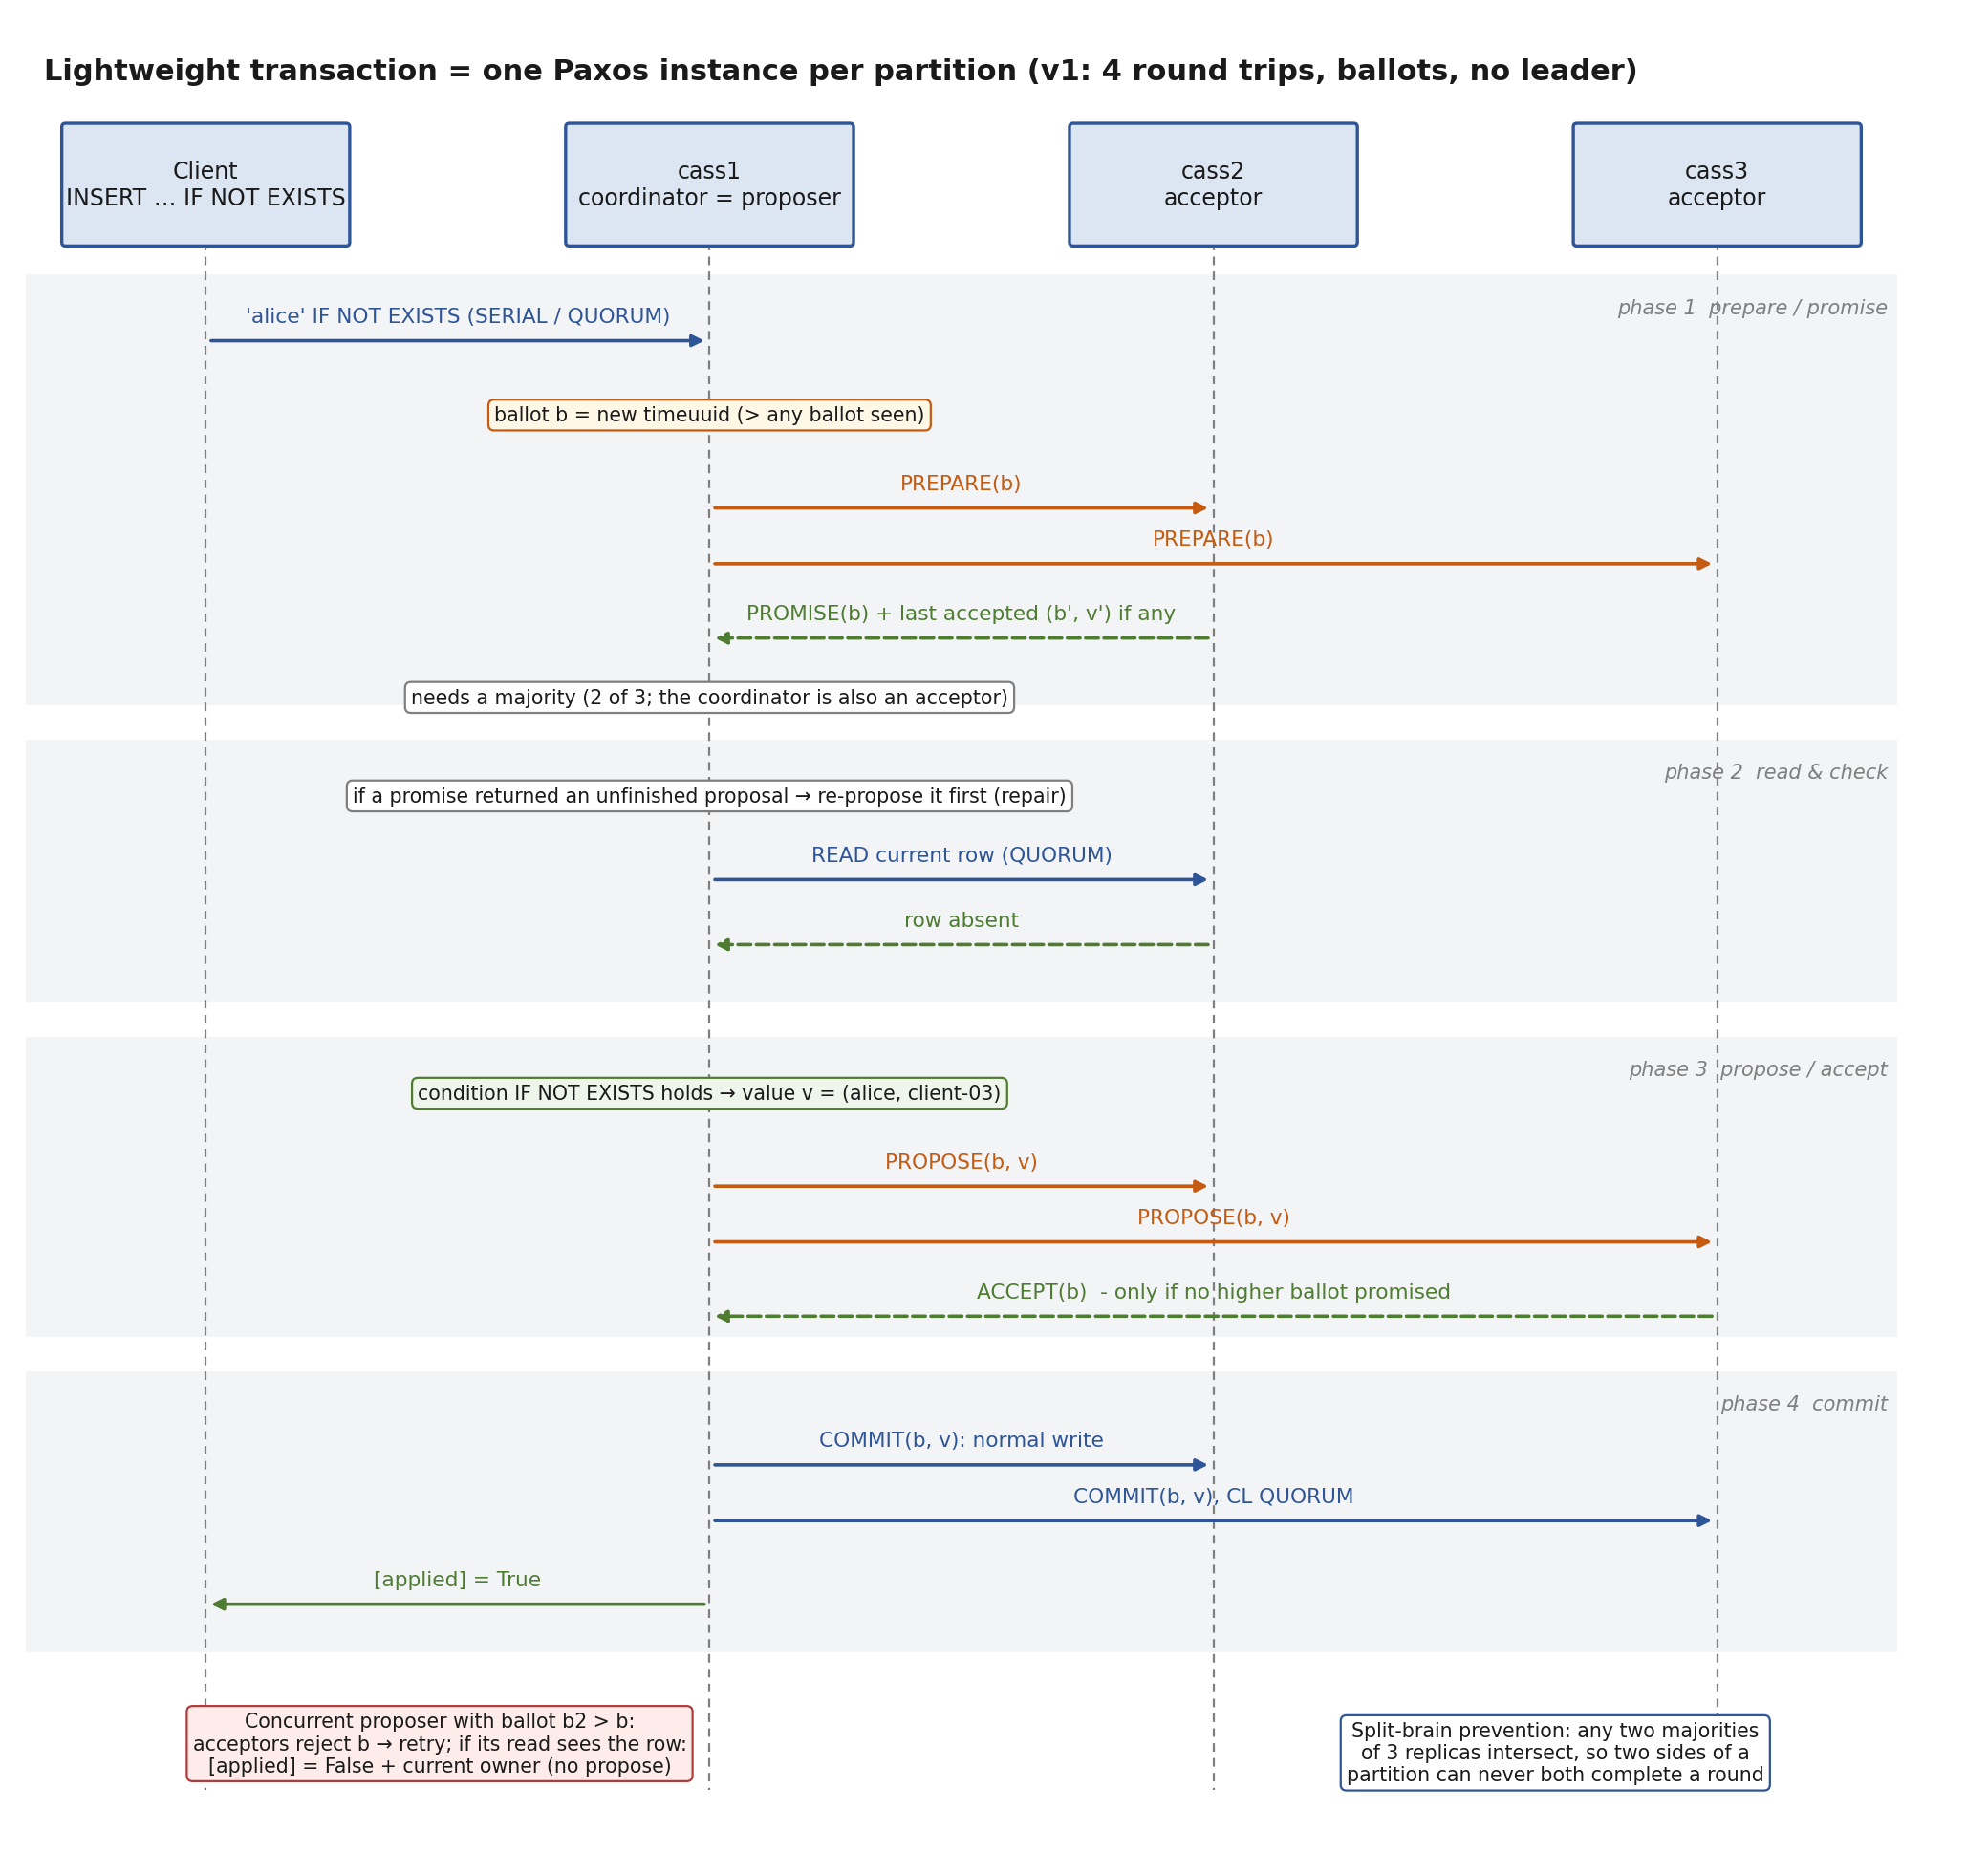
\includegraphics[width=\columnwidth]{paxos_lwt.png}
\caption{One Paxos v1 round of \texttt{INSERT \ldots\ IF NOT EXISTS} on a three-replica
partition; the coordinator is proposer and acceptor. A second proposer loses by ballot order or
sees the row in its read phase.}\label{fig:paxos}
\end{figure}

\subsection{Split-brain prevention}

Any two majorities of $N$ replicas intersect. A Paxos round needs a majority in both the
prepare and the accept phase, so the two sides of a partition can never both complete a round
for the same partition key: the minority side receives \texttt{Unavailable} or a timeout.
With $N = 3$, LWTs survive one failed replica and stop with two---Experiment~6 tests both
cases. Ordinary writes behave differently: at ONE \emph{both} sides of a partition accept
writes, and the divergence is resolved afterwards by LWW (Experiment~5). Cassandra thus does
not prevent split-brain for ordinary data; it tolerates it and reconciles deterministically,
which is what makes it available under partition~\cite{gilbert2002cap,abadi2012pacelc}.
Clients obtain split-brain-free behaviour per operation, by choosing QUORUM/SERIAL.

\subsection{Metadata coordination: gossip (5.0) and TCM (6.0)}

Up to 5.0, schema changes and token ownership also propagate by gossip. A schema change is
applied on one node and spreads as a schema version; nodes can disagree temporarily
(visible in \texttt{nodetool describecluster}---our schema script waits for one version), and
concurrent schema or topology changes can conflict. Cassandra 6.0 replaces this with
Transactional Cluster Metadata (CEP-21~\cite{cep21}): a Cluster Metadata Service keeps a
linearizable, epoch-numbered log of membership, ownership and schema transformations, and
nodes apply entries in log order, so topology changes become multi-step, committed sequences.
6.0 also introduces Accord (CEP-15~\cite{cep15,accord2021}), a leaderless protocol for
multi-partition transactions with strict-serializable isolation that can replace Paxos for
LWTs on migrated tables. At the time of writing 6.0 is a pre-release (6.0-alpha1, a
quarterly alpha for testing only~\cite{cass6alpha}); our measurements describe 5.0 as deployed.

\begin{table}[t]\centering\footnotesize
\setlength{\tabcolsep}{3pt}\caption{Coordination mechanisms and what they guarantee.}\label{tab:coordination}
\begin{tabular}{@{}p{0.26\columnwidth}p{0.2\columnwidth}p{0.16\columnwidth}p{0.25\columnwidth}@{}}\hline
Mechanism & Agreement & Leader & Tolerates ($N=3$) \\ \hline
Gossip / $\varphi$ detector & no (eventual) & none & any failures; views differ \\
Quorum read/write & no (LWW) & none & 1 failure at QUORUM \\
Paxos LWT (5.0) & yes, per partition & none (ballots) & 1 failure \\
TCM / CMS (6.0) & yes, global log & CMS members & minority of CMS \\
Accord (6.0) & yes, multi-partition & none & minority of replicas \\ \hline
\end{tabular}
\end{table}

\setcounter{section}{6}
\section{Experimental Results}
\setcounter{subsection}{3}
% Section 7.4 - Results of Experiments 4 and 6 (Habib Hasanov)
% No typed-in measurement: every value is \expfour{..} / \expsix{..}, defined in
% generated/exp46_numbers.tex by analysis/summarize.py from results/ (make exp4 exp6 figures).
% Until the experiments have run, each value prints as a bold "[run make ...]" marker and the
% figures as a framed placeholder, so a missing run is visible in the PDF.
\providecommand{\expfour}[1]{\ifcsname expfour@#1\endcsname\csname expfour@#1\endcsname\else\textbf{[make exp4]}\fi}
\providecommand{\expsix}[1]{\ifcsname expsix@#1\endcsname\csname expsix@#1\endcsname\else\textbf{[make exp6]}\fi}
\providecommand{\resultfigure}[3]{%
  \IfFileExists{../../results/figures/#1}{\includegraphics[width=#2]{#1}}%
  {\fbox{\parbox{0.9#2}{\centering\footnotesize figure \texttt{\detokenize{#1}} is generated by #3}}}}
\InputIfFileExists{generated/exp46_numbers.tex}{}{}

\subsection{Results: recovery and consensus}\label{sec:results-exp46}

\paragraph{Method (Exp 4)}
\texttt{recovery/hints\_vs\_repair.sh} first runs a full repair so that the cluster starts
converged (baseline preview repair: \expfour{base-preview}), then repeats one fault three times
with a different repair path. cass3 is killed with SIGKILL and, once both peers mark it DN,
\texttt{verify\_convergence write} writes 5\,000 (default) independent keys (one partition each, spread
over all token ranges) at QUORUM and logs every acknowledgement. Freshness on the restarted
replica is measured by reading a fixed sample of 50 keys at ONE \emph{through cass3 as
coordinator} with query tracing on; the trace shows which replica executed the read, so a stale
answer is attributed to cass3 and not to the dynamic snitch's choice. Divergence is measured
without changing data by \texttt{nodetool repair --full --preview}. The final verdict reads
\emph{every} acknowledged key at ALL and passes only if each returns the acknowledged value.
Evidence: \texttt{results/logs/exp4/<run>/}.

\paragraph{4a: hinted handoff}
While cass3 was down, \expfour{4a-acked} of \expfour{4a-written} writes were acknowledged and
the two coordinators accumulated \expfour{4a-hint-files} hint files
(\expfour{4a-hint-kib}\,KiB). After \texttt{docker start}, peers saw cass3 Up/Normal after
\expfour{4a-un-s}\,s and the hint files were gone \expfour{4a-drain-s}\,s later
(Fig.~\ref{fig:hints}; dispatch log lines in \texttt{4a\_04\_hint\_dispatch\_log.txt}). Without
any manual repair the preview repair then reported \expfour{4a-preview}, and
\expfour{4a-one-stale} of \expfour{4a-one-checked} sample reads served by cass3 were stale.
\expfour{4a-conclusion} Verdict: \expfour{4a-verdict}.

\paragraph{4b: read repair only}
With \texttt{nodetool disablehandoff} on cass1 and cass2, the same outage left cass3 without
the \expfour{4b-acked} acknowledged writes: after restart the preview repair found
\expfour{4b-preview-ranges} divergent ranges (\expfour{4b-preview-kib}\,KiB to stream), and
\expfour{4b-before-target-stale} of the \expfour{4b-before-target} sample reads executed by
cass3 at ONE were stale---the replica answered from its own incomplete data, which no ONE read
can detect. Reading the same 50 keys once at ALL produced traces with a digest mismatch / read
repair for \expfour{4b-all-repair-traces} keys; afterwards \expfour{4b-after-stale} of
\expfour{4b-after-checked} ONE reads from cass3 were stale. A disjoint control sample that was
never read at ALL remained stale (\expfour{4b-control-stale} of \expfour{4b-control-checked}),
and a second preview still reported \expfour{4b2-preview} (\expfour{4b2-preview-kib}\,KiB).
\expfour{4b-conclusion}

\paragraph{4c: anti-entropy repair}
\texttt{nodetool repair --full chat} on cass3 took \expfour{4c-repair-s}\,s. The preview then
reported \expfour{4c-preview}, the control sample was stale in \expfour{4c-control-stale} of
\expfour{4c-control-checked} reads, and all \expfour{4c-acked-checked} acknowledged writes of 4a
and 4b were read back at ALL with their acknowledged value (missing: \expfour{4c-acked-missing},
wrong: \expfour{4c-acked-wrong}). \expfour{4c-conclusion} Convergence verdict:
\textbf{\expfour{4c-verdict}}.

\begin{figure}[t]\centering
\resultfigure{exp4_hints_drain.png}{\columnwidth}{make exp4 \&\& make figures}
\caption{Exp 4a: hint files held by cass1 and cass2 after the dead replica is restarted; the
dashed line marks the moment peers report it Up/Normal.}\label{fig:hints}
\end{figure}

\paragraph{Method (Exp 6)}
\texttt{recovery/lwt\_demo.py} releases \expsix{race-clients} threads through a barrier so that
they claim the same handle at the same instant, for \expsix{race-handles} handles, once with
\texttt{INSERT \ldots\ IF NOT EXISTS} (serial SERIAL, commit QUORUM) and once with a plain
QUORUM \texttt{INSERT}. After each handle the owner is read back at SERIAL.

\paragraph{Exp 6 results}
With LWTs, \expsix{race-exactlyone} of \expsix{race-handles} handles were classified
\emph{exactly one winner} (one \texttt{[applied] = True}, every loser told the winner's owner,
the SERIAL read-back agreeing); \expsix{race-timeoutwinner} winners were LWTs that timed out
but had committed, and \expsix{race-violations} handles had more than one winner.
\expsix{race-conclusion} With plain inserts all \expsix{plain-opsok}
operations were acknowledged and \expsix{plain-ackedoverwritten} of them were silently
overwritten (Section~\ref{sec:consensus}). Consensus is not free: over \expsix{lat-lwt-n}
sequential uncontended inserts the LWT median was \expsix{lat-lwt-p50}\,ms (p99
\expsix{lat-lwt-p99}) against \expsix{lat-plain-p50}\,ms (p99 \expsix{lat-plain-p99}) for a
plain QUORUM write, a factor of \expsix{lat-ratio} (Fig.~\ref{fig:lwt}), \expsix{lat-conclusion}. With cass3 down, \expsix{race1-exactlyone} of
\expsix{race1-handles} handles still had exactly one winner, since two of three replicas form a
Paxos majority. With cass2 and cass3 down no LWT could complete (\expsix{race2-nowinner} of
\expsix{race2-handles} handles without a winner; errors: \expsix{race2-errors}) and no handle had
more than one winner (\expsix{race2-violations}). \expsix{race2-conclusion}

\begin{figure}[t]\centering
\resultfigure{exp6_lwt_latency.png}{\columnwidth}{make exp6 \&\& make figures}
\caption{Exp 6: latency distribution of uncontended LWT inserts vs.\ plain QUORUM inserts.}
\label{fig:lwt}
\end{figure}

\paragraph{Limitations}
All nodes share one host: network latency is sub-millisecond and identical between replicas,
so the absolute LWT cost underestimates a multi-rack or WAN deployment, where each extra round
trip costs a network RTT. The outage in Exp 4 lasts tens of seconds, far below
\texttt{max\_hint\_window}; hints were therefore complete, which is the favourable case. The
preview repair estimates streaming at Merkle-leaf granularity, so its byte count is an upper
bound on the data actually missing.

\subsection*{Contribution to Section 7.3 (fault-phase analysis of Exp 3 and 5)}
% Fault-phase availability analysis of Exp 3 and Exp 5 (Habib Hasanov, results analysis owner).
% Offered to Person 3 for \input in section 7.3 (or section 6). Every value comes from
% analysis/summarize.py: \expfault{..} in generated/exp46_numbers.tex, Table~\ref{tab:fault-phases}
% and Table~\ref{tab:detection} in generated/fault_tables.tex, and the figure from analysis/plots.py.
\providecommand{\expfault}[1]{\ifcsname expfault@#1\endcsname\csname expfault@#1\endcsname\else\textbf{[make figures]}\fi}
\InputIfFileExists{generated/exp46_numbers.tex}{}{}

\subsubsection*{Availability inside the fault window}
Whole-run success rates mix healthy and faulty periods. Splitting the availability-probe
operations of Exp 3 and Exp 5 at the injection and restart/heal commands in
\texttt{results/logs/chaos\_events.csv} isolates the fault window
(Table~\ref{tab:fault-phases}, Fig.~\ref{fig:fault-timeline}). With one node killed (3a), ONE
and QUORUM kept \expfault{3a-fault-ONE}\,\% and \expfault{3a-fault-QUORUM}\,\% success while ALL
dropped to \expfault{3a-fault-ALL}\,\%: first as timeouts until gossip declared the node down
(about \expfault{det-kill}\,s), then as immediate \texttt{Unavailable}. In 3b the second kill
followed the first by about 19\,s, so QUORUM succeeded until the second node failed and
\expfault{3b-fault-QUORUM}\,\% over the whole window, while ONE stayed at
\expfault{3b-fault-ONE}\,\%. ALL recovered only some seconds \emph{after} the restart command,
when the node had rejoined, so the ``after'' phase still contains failures.

\paragraph{Client-side unavailability under partition}
In Exp 5 the server-side behaviour matched the design (the majority accepted QUORUM writes),
but in each of the \expfault{exp5-stuck-runs} repetitions one probe level whose key had cass3
as first replica (\expfault{exp5-stuck-levels}) sent its requests to the isolated cass3 and
waited for the 5\,s client timeout, \expfault{exp5-stuck-timeouts} times in total, until the
partition healed. Every one of these requests was coordinated by cass3; a disconnected
container drops packets without resetting the client's TCP connections, which is the likely
reason the driver kept routing to it, and with retries disabled each such request failed. Pooled over repetitions
this is hidden (ONE \expfault{partition-fault-ONE}\,\%, QUORUM \expfault{partition-fault-QUORUM}\,\%),
but for the affected client the level was unavailable for over a minute although the cluster
could serve it. Availability in the CAP sense is therefore a property of the client's route as
well as of the replica set; a retry or speculative-execution policy that moves to the next
replica after a timeout would have masked it.

% Generated by analysis/summarize.py - do not edit by hand.
\begin{table}[t]\centering\footnotesize\setlength{\tabcolsep}{3pt}
\caption{Availability-probe success rate per consistency level and fault phase (Exp 3 and 5; repetitions pooled; ``fault'' = from the injection command to the restart/heal command).}\label{tab:fault-phases}
\begin{tabular}{llrrr}\hline
Run & Phase & ONE (\%) & QUORUM (\%) & ALL (\%) \\ \hline
exp3 3a & before & 100.0 & 100.0 & 100.0 \\
exp3 3a & fault & 100.0 & 100.0 & 4.7 \\
exp3 3a & after & 100.0 & 100.0 & 92.1 \\
exp3 3b & before & 100.0 & 100.0 & 100.0 \\
exp3 3b & fault & 99.9 & 60.1 & 2.0 \\
exp3 3b & after & 100.0 & 100.0 & 82.2 \\
exp3 3c & before & 100.0 & 100.0 & 100.0 \\
exp3 3c & fault & 100.0 & 100.0 & 5.3 \\
exp3 3c & between & 100.0 & 100.0 & 64.2 \\
exp3 3c & after & 100.0 & 100.0 & 93.9 \\
exp5 partition & before & 100.0 & 100.0 & 100.0 \\
exp5 partition & fault & 95.6 & 98.8 & 7.1 \\
exp5 partition & after & 98.9 & 99.5 & 98.3 \\
\hline\end{tabular}\end{table}

\begin{table}[t]\centering\footnotesize\setlength{\tabcolsep}{3pt}
\caption{Gossip failure-detection time (fault command to ``is now DOWN/UP'' in a peer's log).}\label{tab:detection}
\begin{tabular}{lrrrr}\hline
Fault (transition) & $n$ & mean (s) & min (s) & max (s) \\ \hline
kill (down) & 13 & 19.63 & 18.87 & 22.19 \\
partition, majority view & 4 & 19.19 & 18.75 & 19.38 \\
partition, minority view & 4 & 18.75 & 18.10 & 19.24 \\
start (up) & 16 & 9.85 & 7.25 & 11.12 \\
stop (down) & 3 & 0.67 & 0.54 & 0.81 \\
\hline\end{tabular}\end{table}



\begin{figure*}[t]\centering
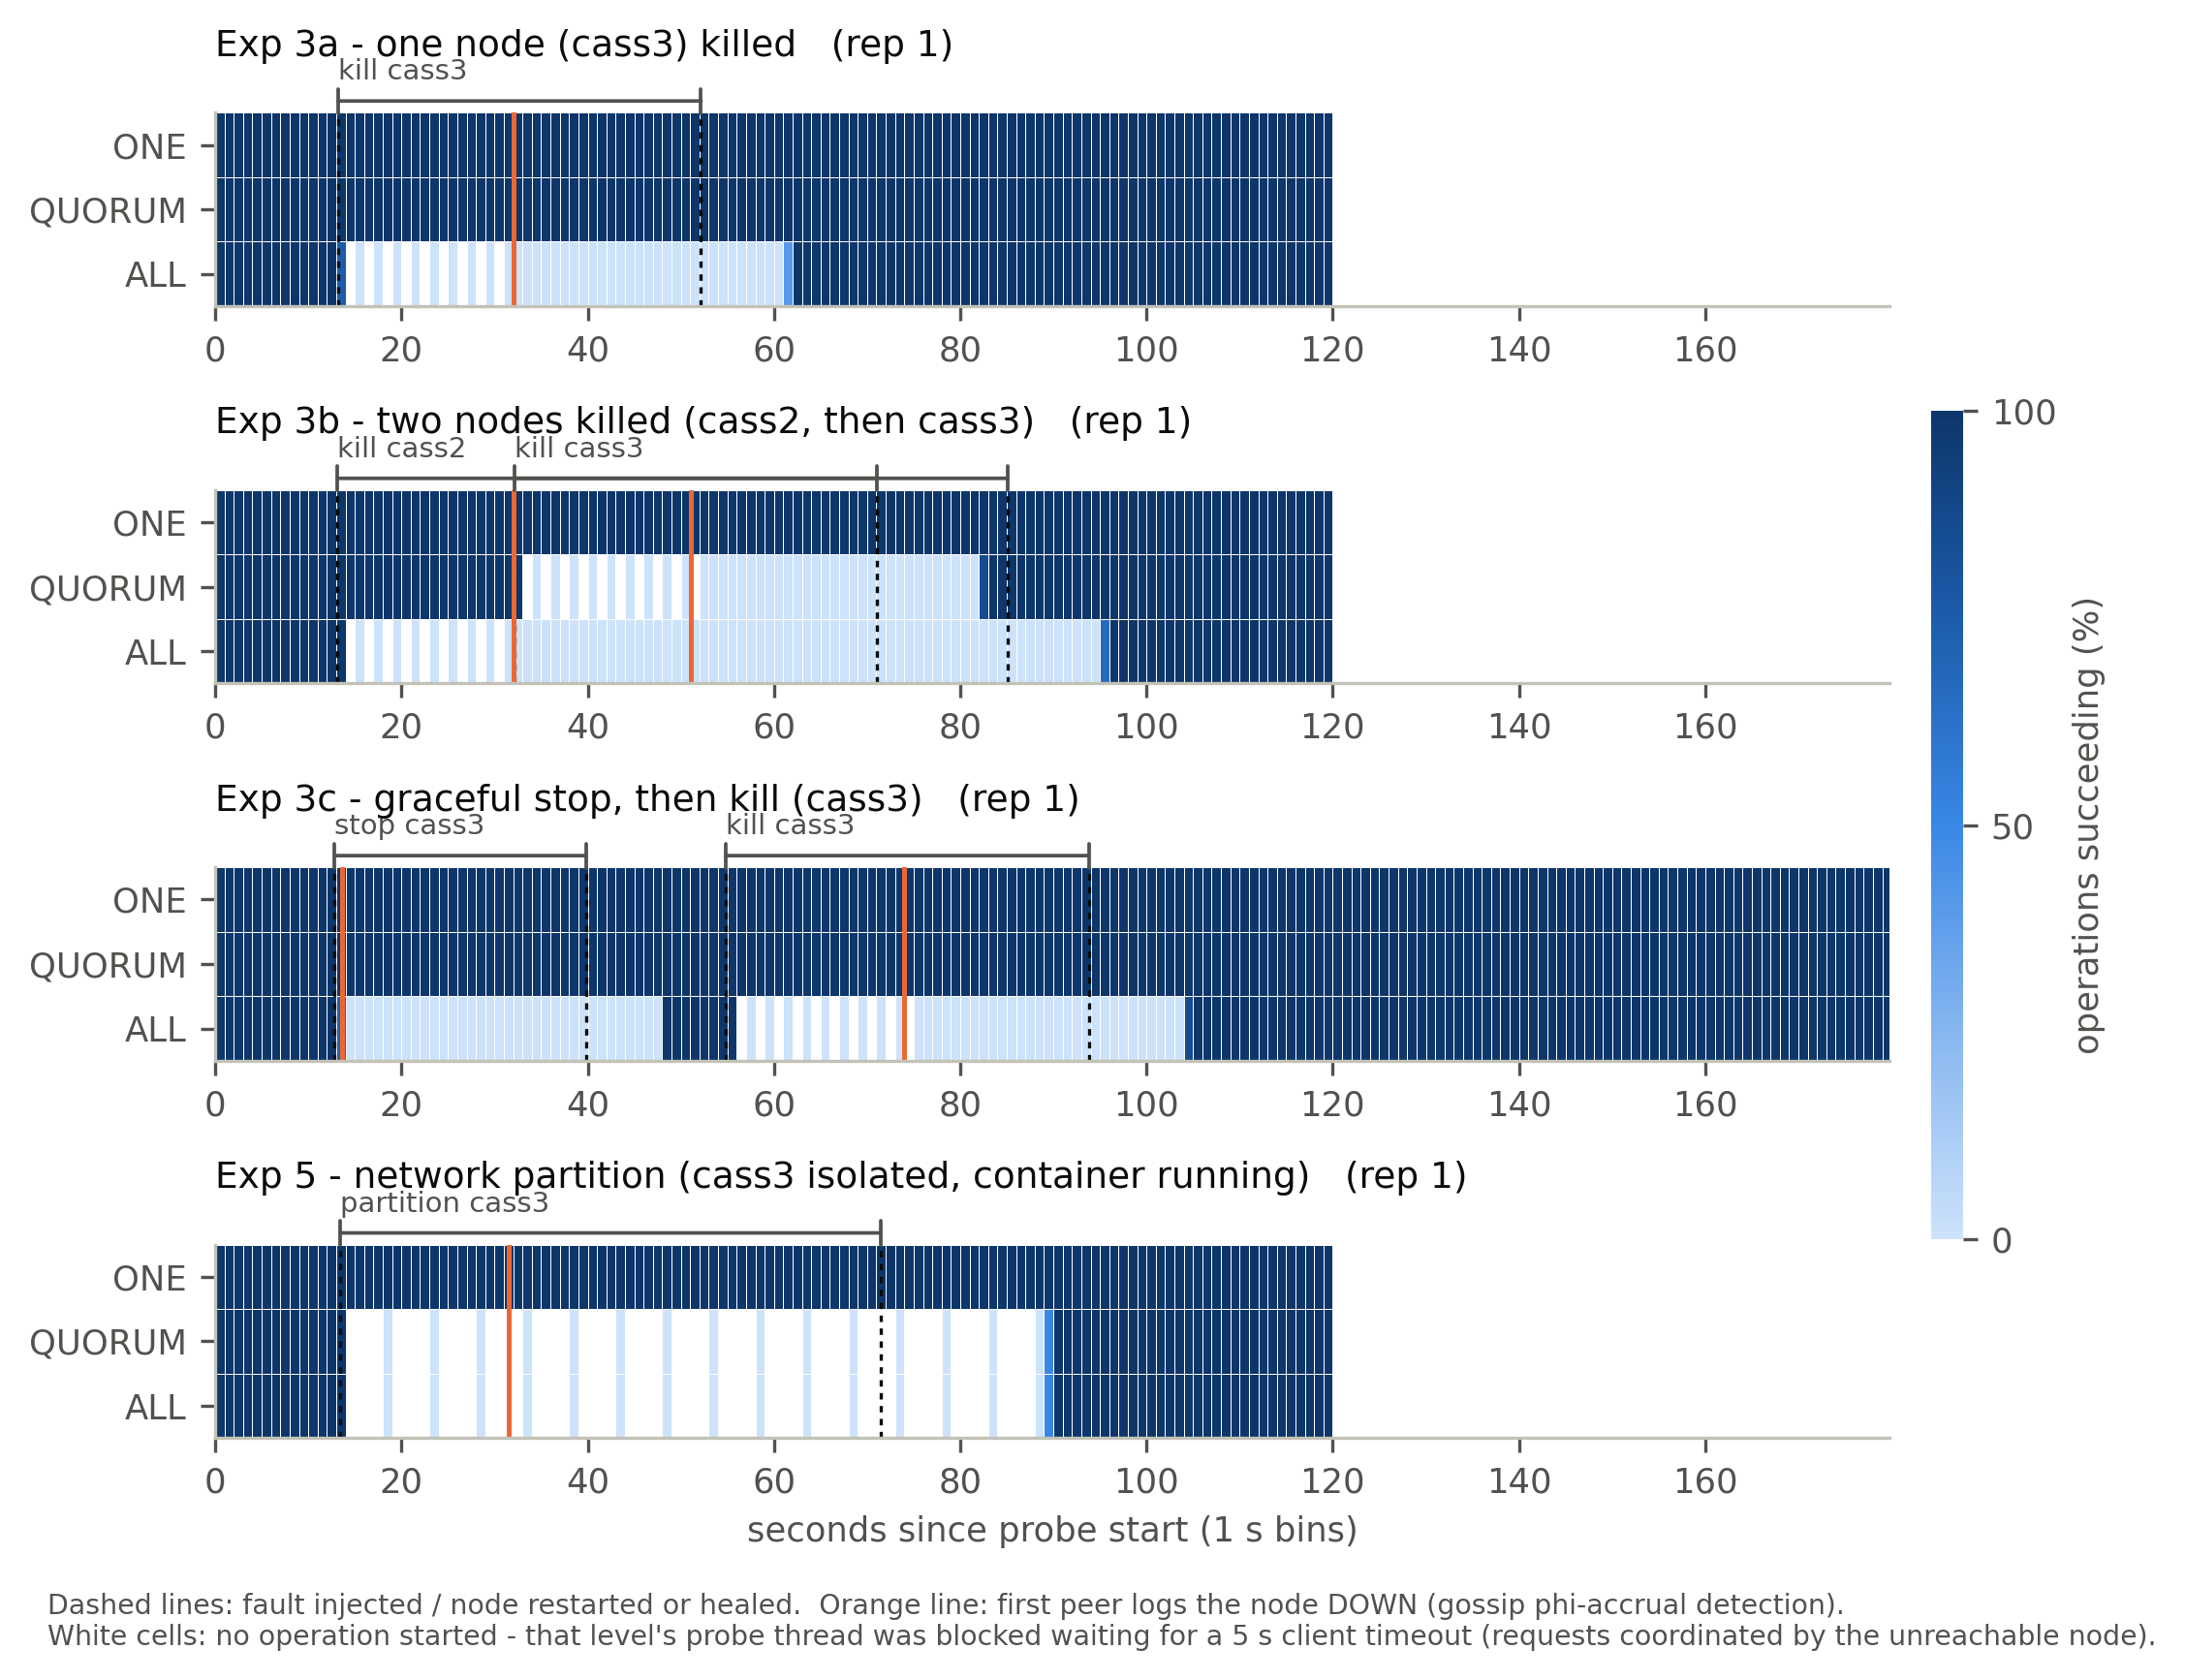
\includegraphics[width=\textwidth]{fault_availability_timeline.png}
\caption{Per-second success of the ONE/QUORUM/ALL availability probe in repetition 1 of each
fault scenario. Dashed lines: fault injected and node restarted/healed; orange: first peer
logs the node DOWN. White cells: the probe of that level was blocked on a 5\,s client
timeout.}\label{fig:fault-timeline}
\end{figure*}

\bibliographystyle{ieeetr}
\bibliography{references}
\end{document}
